\documentclass{standalone}
\usepackage{tikz}
\usetikzlibrary{patterns, positioning}

\begin{document}
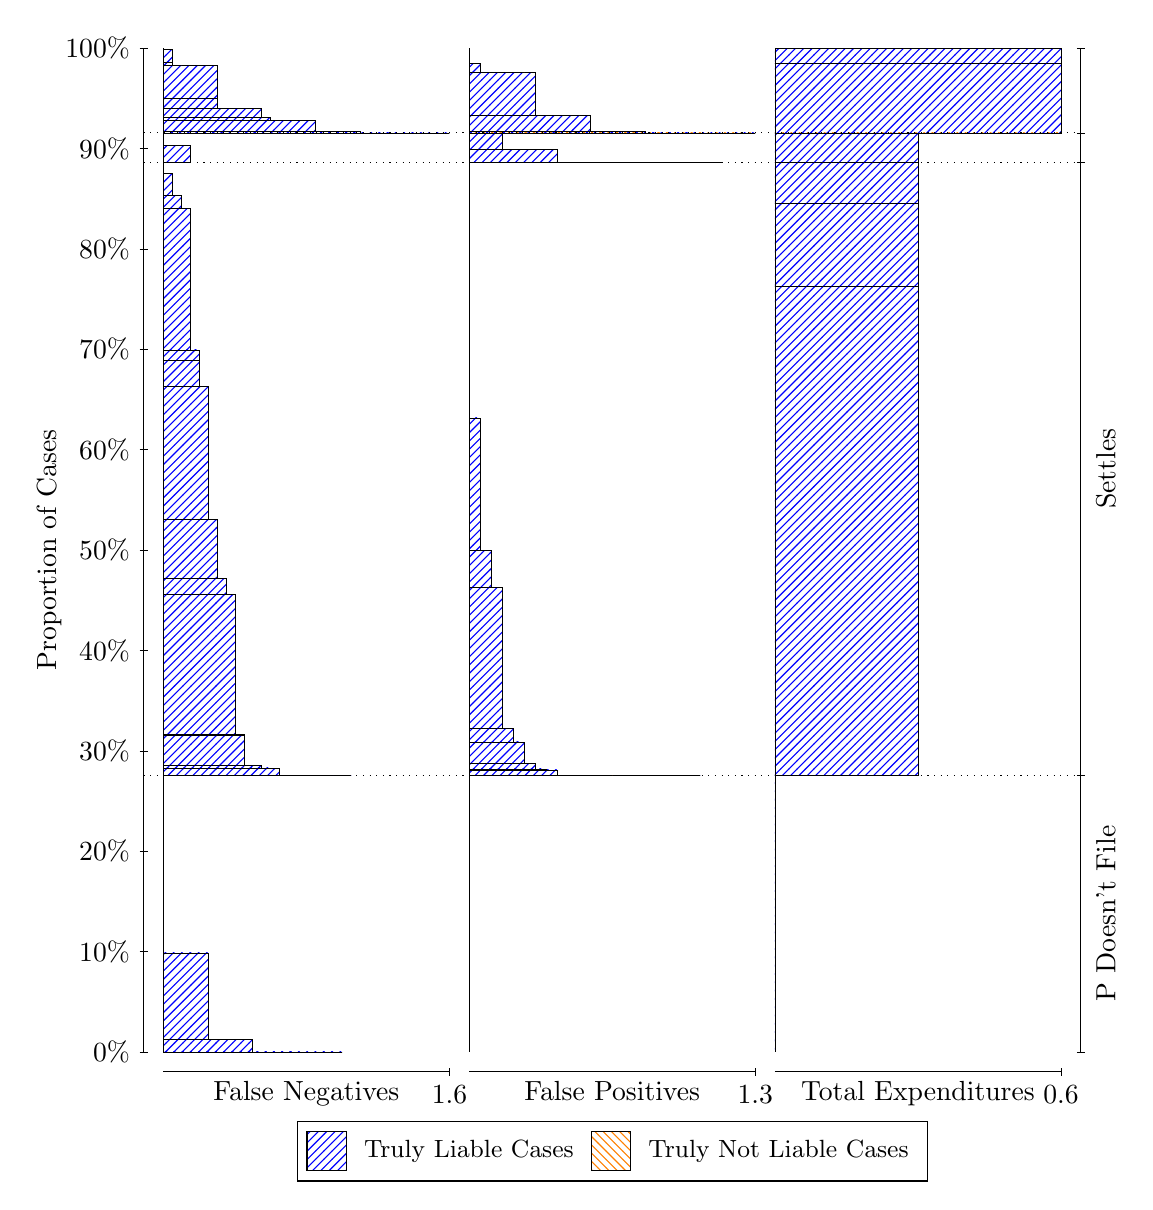
\begin{tikzpicture}
\draw[black, very thin] (1.5,1.75) -- (1.5,14.5);
\node[rotate=90, anchor=center] at (0.3, 8.125) {Proportion of Cases};
\draw[black, very thin] (1.45,1.75) -- (1.55,1.75);
\node[anchor=east] at (1.45, 1.75) {0\%};
\draw[black, very thin] (1.45,3.025) -- (1.55,3.025);
\node[anchor=east] at (1.45, 3.025) {10\%};
\draw[black, very thin] (1.45,4.3) -- (1.55,4.3);
\node[anchor=east] at (1.45, 4.3) {20\%};
\draw[black, very thin] (1.45,5.575) -- (1.55,5.575);
\node[anchor=east] at (1.45, 5.575) {30\%};
\draw[black, very thin] (1.45,6.85) -- (1.55,6.85);
\node[anchor=east] at (1.45, 6.85) {40\%};
\draw[black, very thin] (1.45,8.125) -- (1.55,8.125);
\node[anchor=east] at (1.45, 8.125) {50\%};
\draw[black, very thin] (1.45,9.4) -- (1.55,9.4);
\node[anchor=east] at (1.45, 9.4) {60\%};
\draw[black, very thin] (1.45,10.675) -- (1.55,10.675);
\node[anchor=east] at (1.45, 10.675) {70\%};
\draw[black, very thin] (1.45,11.95) -- (1.55,11.95);
\node[anchor=east] at (1.45, 11.95) {80\%};
\draw[black, very thin] (1.45,13.225) -- (1.55,13.225);
\node[anchor=east] at (1.45, 13.225) {90\%};
\draw[black, very thin] (1.45,14.5) -- (1.55,14.5);
\node[anchor=east] at (1.45, 14.5) {100\%};

\draw[black, very thin] (13.4,1.75) -- (13.4,14.5);
\draw[black, very thin] (13.35,1.75) -- (13.45,1.75);
\node[anchor=west] at (13.35, 1.75) {};
\draw[black, very thin] (13.35,5.2666) -- (13.45,5.2666);
\node[anchor=west] at (13.35, 5.2666) {};
\draw[black, very thin] (13.35,13.05) -- (13.45,13.05);
\node[anchor=west] at (13.35, 13.05) {};
\draw[black, very thin] (13.35,13.422) -- (13.45,13.422);
\node[anchor=west] at (13.35, 13.422) {};
\draw[black, very thin] (13.35,14.5) -- (13.45,14.5);
\node[anchor=west] at (13.35, 14.5) {};

\draw[black, very thin, pattern color=blue, pattern=north east lines] (1.75,1.75) rectangle (4.0208,1.75);
\draw[black, very thin, pattern color=blue, pattern=north east lines] (1.75,1.75) rectangle (3.4531,1.7514);
\draw[black, very thin, pattern color=blue, pattern=north east lines] (1.75,1.7514) rectangle (2.8854,1.9141);
\draw[black, very thin, pattern color=blue, pattern=north east lines] (1.75,1.9141) rectangle (2.3177,3.0081);
\draw[black, very thin, pattern color=orange, pattern=north west lines] (1.75,3.0081) rectangle (1.75,3.0081);
\draw[black, very thin, pattern color=blue, pattern=north east lines] (1.75,3.0081) rectangle (1.75,5.2666);
\draw[black, very thin, pattern color=blue, pattern=north east lines] (1.75,5.2666) rectangle (4.1344,5.2666);
\draw[black, very thin, pattern color=blue, pattern=north east lines] (1.75,5.2666) rectangle (3.9073,5.2666);
\draw[black, very thin, pattern color=blue, pattern=north east lines] (1.75,5.2666) rectangle (3.6802,5.2666);
\draw[black, very thin, pattern color=blue, pattern=north east lines] (1.75,5.2666) rectangle (3.5667,5.2666);
\draw[black, very thin, pattern color=blue, pattern=north east lines] (1.75,5.2666) rectangle (3.3396,5.2666);
\draw[black, very thin, pattern color=blue, pattern=north east lines] (1.75,5.2666) rectangle (3.226,5.3558);
\draw[black, very thin, pattern color=blue, pattern=north east lines] (1.75,5.3558) rectangle (3.1125,5.3576);
\draw[black, very thin, pattern color=blue, pattern=north east lines] (1.75,5.3576) rectangle (2.999,5.3888);
\draw[black, very thin, pattern color=blue, pattern=north east lines] (1.75,5.3888) rectangle (2.7719,5.7728);
\draw[black, very thin, pattern color=blue, pattern=north east lines] (1.75,5.7728) rectangle (2.7719,5.7799);
\draw[black, very thin, pattern color=blue, pattern=north east lines] (1.75,5.7799) rectangle (2.6583,7.5608);
\draw[black, very thin, pattern color=blue, pattern=north east lines] (1.75,7.5608) rectangle (2.5448,7.7639);
\draw[black, very thin, pattern color=blue, pattern=north east lines] (1.75,7.7639) rectangle (2.4312,8.5135);
\draw[black, very thin, pattern color=blue, pattern=north east lines] (1.75,8.5135) rectangle (2.3177,10.199);
\draw[black, very thin, pattern color=blue, pattern=north east lines] (1.75,10.199) rectangle (2.2042,10.532);
\draw[black, very thin, pattern color=blue, pattern=north east lines] (1.75,10.532) rectangle (2.2042,10.666);
\draw[black, very thin, pattern color=blue, pattern=north east lines] (1.75,10.666) rectangle (2.0906,12.461);
\draw[black, very thin, pattern color=blue, pattern=north east lines] (1.75,12.461) rectangle (1.9771,12.628);
\draw[black, very thin, pattern color=blue, pattern=north east lines] (1.75,12.628) rectangle (1.8635,12.905);
\draw[black, very thin, pattern color=orange, pattern=north west lines] (1.75,12.905) rectangle (1.75,12.905);
\draw[black, very thin, pattern color=blue, pattern=north east lines] (1.75,12.905) rectangle (1.75,13.05);
\draw[black, very thin, pattern color=blue, pattern=north east lines] (1.75,13.05) rectangle (2.0906,13.261);
\draw[black, very thin, pattern color=orange, pattern=north west lines] (1.75,13.261) rectangle (1.75,13.261);
\draw[black, very thin, pattern color=blue, pattern=north east lines] (1.75,13.261) rectangle (1.75,13.422);
\draw[black, very thin, pattern color=blue, pattern=north east lines] (1.75,13.422) rectangle (5.3833,13.422);
\draw[black, very thin, pattern color=blue, pattern=north east lines] (1.75,13.422) rectangle (4.8156,13.423);
\draw[black, very thin, pattern color=blue, pattern=north east lines] (1.75,13.423) rectangle (4.2479,13.44);
\draw[black, very thin, pattern color=blue, pattern=north east lines] (1.75,13.44) rectangle (4.1344,13.44);
\draw[black, very thin, pattern color=blue, pattern=north east lines] (1.75,13.44) rectangle (3.6802,13.584);
\draw[black, very thin, pattern color=blue, pattern=north east lines] (1.75,13.584) rectangle (3.5667,13.584);
\draw[black, very thin, pattern color=blue, pattern=north east lines] (1.75,13.584) rectangle (3.1125,13.617);
\draw[black, very thin, pattern color=blue, pattern=north east lines] (1.75,13.617) rectangle (2.999,13.737);
\draw[black, very thin, pattern color=blue, pattern=north east lines] (1.75,13.737) rectangle (2.5448,13.737);
\draw[black, very thin, pattern color=blue, pattern=north east lines] (1.75,13.737) rectangle (2.4312,13.856);
\draw[black, very thin, pattern color=blue, pattern=north east lines] (1.75,13.856) rectangle (2.4312,14.275);
\draw[black, very thin, pattern color=blue, pattern=north east lines] (1.75,14.275) rectangle (1.9771,14.275);
\draw[black, very thin, pattern color=blue, pattern=north east lines] (1.75,14.275) rectangle (1.8635,14.323);
\draw[black, very thin, pattern color=blue, pattern=north east lines] (1.75,14.323) rectangle (1.8635,14.484);
\draw[black, very thin, pattern color=orange, pattern=north west lines] (1.75,14.484) rectangle (1.75,14.484);
\draw[black, very thin, pattern color=blue, pattern=north east lines] (1.75,14.484) rectangle (1.75,14.5);
\draw[black, very thin, pattern color=orange, pattern=north west lines] (5.6333,1.75) rectangle (5.6333,1.75);
\draw[black, very thin, pattern color=blue, pattern=north east lines] (5.6333,1.75) rectangle (5.6333,5.2666);
\draw[black, very thin, pattern color=orange, pattern=north west lines] (5.6333,5.2666) rectangle (8.5679,5.2666);
\draw[black, very thin, pattern color=blue, pattern=north east lines] (5.6333,5.2666) rectangle (8.5679,5.2666);
\draw[black, very thin, pattern color=orange, pattern=north west lines] (5.6333,5.2666) rectangle (8.009,5.2666);
\draw[black, very thin, pattern color=blue, pattern=north east lines] (5.6333,5.2666) rectangle (8.009,5.2666);
\draw[black, very thin, pattern color=blue, pattern=north east lines] (5.6333,5.2666) rectangle (7.8692,5.2666);
\draw[black, very thin, pattern color=orange, pattern=north west lines] (5.6333,5.2666) rectangle (7.45,5.2666);
\draw[black, very thin, pattern color=blue, pattern=north east lines] (5.6333,5.2666) rectangle (7.45,5.2666);
\draw[black, very thin, pattern color=blue, pattern=north east lines] (5.6333,5.2666) rectangle (7.3103,5.2666);
\draw[black, very thin, pattern color=blue, pattern=north east lines] (5.6333,5.2666) rectangle (7.1705,5.2666);
\draw[black, very thin, pattern color=orange, pattern=north west lines] (5.6333,5.2666) rectangle (6.891,5.2666);
\draw[black, very thin, pattern color=blue, pattern=north east lines] (5.6333,5.2666) rectangle (6.891,5.2671);
\draw[black, very thin, pattern color=blue, pattern=north east lines] (5.6333,5.2671) rectangle (6.7513,5.3314);
\draw[black, very thin, pattern color=orange, pattern=north west lines] (5.6333,5.3314) rectangle (6.6115,5.3314);
\draw[black, very thin, pattern color=blue, pattern=north east lines] (5.6333,5.3314) rectangle (6.6115,5.3444);
\draw[black, very thin, pattern color=blue, pattern=north east lines] (5.6333,5.3444) rectangle (6.4718,5.4121);
\draw[black, very thin, pattern color=orange, pattern=north west lines] (5.6333,5.4121) rectangle (6.3321,5.4121);
\draw[black, very thin, pattern color=blue, pattern=north east lines] (5.6333,5.4121) rectangle (6.3321,5.689);
\draw[black, very thin, pattern color=blue, pattern=north east lines] (5.6333,5.689) rectangle (6.1923,5.8559);
\draw[black, very thin, pattern color=blue, pattern=north east lines] (5.6333,5.8559) rectangle (6.0526,7.6501);
\draw[black, very thin, pattern color=blue, pattern=north east lines] (5.6333,7.6501) rectangle (5.9128,8.118);
\draw[black, very thin, pattern color=blue, pattern=north east lines] (5.6333,8.118) rectangle (5.7731,9.8032);
\draw[black, very thin, pattern color=blue, pattern=north east lines] (5.6333,9.8032) rectangle (5.6333,13.05);
\draw[black, very thin, pattern color=orange, pattern=north west lines] (5.6333,13.05) rectangle (8.8474,13.05);
\draw[black, very thin, pattern color=blue, pattern=north east lines] (5.6333,13.05) rectangle (8.8474,13.05);
\draw[black, very thin, pattern color=blue, pattern=north east lines] (5.6333,13.05) rectangle (8.1487,13.05);
\draw[black, very thin, pattern color=blue, pattern=north east lines] (5.6333,13.05) rectangle (7.45,13.051);
\draw[black, very thin, pattern color=blue, pattern=north east lines] (5.6333,13.051) rectangle (6.7513,13.211);
\draw[black, very thin, pattern color=blue, pattern=north east lines] (5.6333,13.211) rectangle (6.0526,13.422);
\draw[black, very thin, pattern color=orange, pattern=north west lines] (5.6333,13.422) rectangle (9.2667,13.422);
\draw[black, very thin, pattern color=blue, pattern=north east lines] (5.6333,13.422) rectangle (9.2667,13.422);
\draw[black, very thin, pattern color=orange, pattern=north west lines] (5.6333,13.422) rectangle (8.5679,13.422);
\draw[black, very thin, pattern color=blue, pattern=north east lines] (5.6333,13.422) rectangle (8.5679,13.422);
\draw[black, very thin, pattern color=orange, pattern=north west lines] (5.6333,13.422) rectangle (7.8692,13.422);
\draw[black, very thin, pattern color=blue, pattern=north east lines] (5.6333,13.422) rectangle (7.8692,13.438);
\draw[black, very thin, pattern color=orange, pattern=north west lines] (5.6333,13.438) rectangle (7.1705,13.438);
\draw[black, very thin, pattern color=blue, pattern=north east lines] (5.6333,13.438) rectangle (7.1705,13.648);
\draw[black, very thin, pattern color=orange, pattern=north west lines] (5.6333,13.648) rectangle (7.0308,13.648);
\draw[black, very thin, pattern color=blue, pattern=north east lines] (5.6333,13.648) rectangle (7.0308,13.648);
\draw[black, very thin, pattern color=blue, pattern=north east lines] (5.6333,13.648) rectangle (6.4718,14.186);
\draw[black, very thin, pattern color=orange, pattern=north west lines] (5.6333,14.186) rectangle (6.3321,14.186);
\draw[black, very thin, pattern color=blue, pattern=north east lines] (5.6333,14.186) rectangle (6.3321,14.186);
\draw[black, very thin, pattern color=blue, pattern=north east lines] (5.6333,14.186) rectangle (5.7731,14.306);
\draw[black, very thin, pattern color=orange, pattern=north west lines] (5.6333,14.306) rectangle (5.6333,14.306);
\draw[black, very thin, pattern color=blue, pattern=north east lines] (5.6333,14.306) rectangle (5.6333,14.5);
\draw[black, very thin, pattern color=orange, pattern=north west lines] (9.5167,1.75) rectangle (9.5167,1.75);
\draw[black, very thin, pattern color=blue, pattern=north east lines] (9.5167,1.75) rectangle (9.5167,5.2666);
\draw[black, very thin, pattern color=orange, pattern=north west lines] (9.5167,5.2666) rectangle (11.333,5.2666);
\draw[black, very thin, pattern color=blue, pattern=north east lines] (9.5167,5.2666) rectangle (11.333,11.468);
\draw[black, very thin, pattern color=orange, pattern=north west lines] (9.5167,11.468) rectangle (11.333,11.468);
\draw[black, very thin, pattern color=blue, pattern=north east lines] (9.5167,11.468) rectangle (11.333,12.526);
\draw[black, very thin, pattern color=orange, pattern=north west lines] (9.5167,12.526) rectangle (11.333,12.526);
\draw[black, very thin, pattern color=blue, pattern=north east lines] (9.5167,12.526) rectangle (11.333,13.05);
\draw[black, very thin, pattern color=orange, pattern=north west lines] (9.5167,13.05) rectangle (11.333,13.05);
\draw[black, very thin, pattern color=blue, pattern=north east lines] (9.5167,13.05) rectangle (11.333,13.422);
\draw[black, very thin, pattern color=orange, pattern=north west lines] (9.5167,13.422) rectangle (13.15,13.422);
\draw[black, very thin, pattern color=blue, pattern=north east lines] (9.5167,13.422) rectangle (13.15,14.306);
\draw[black, very thin, pattern color=orange, pattern=north west lines] (9.5167,14.306) rectangle (13.15,14.306);
\draw[black, very thin, pattern color=blue, pattern=north east lines] (9.5167,14.306) rectangle (13.15,14.5);
\draw[black, dotted] (1.5,5.2666) -- (13.4,5.2666);
\draw[black, dotted] (1.5,13.05) -- (13.4,13.05);
\draw[black, dotted] (1.5,13.422) -- (13.4,13.422);
\draw[black, very thin] (1.75,1.5) -- (5.3833,1.5);
\node[anchor=north] at (3.5667, 1.5) {False Negatives};
\draw[black, very thin] (5.3833,1.45) -- (5.3833,1.55);
\node[anchor=north] at (5.3833, 1.45) {1.6};

\draw[black, very thin] (5.6333,1.5) -- (9.2667,1.5);
\node[anchor=north] at (7.45, 1.5) {False Positives};
\draw[black, very thin] (9.2667,1.45) -- (9.2667,1.55);
\node[anchor=north] at (9.2667, 1.45) {1.3};

\draw[black, very thin] (9.5167,1.5) -- (13.15,1.5);
\node[anchor=north] at (11.333, 1.5) {Total Expenditures};
\draw[black, very thin] (13.15,1.45) -- (13.15,1.55);
\node[anchor=north] at (13.15, 1.45) {0.6};

\node[black, centered, rotate=90] at (13.72, 3.5083) {P Doesn't File};
\node[black, centered, rotate=90] at (13.72, 9.1583) {Settles};



\draw (7.449999999999999,1.5) node[draw=none] (baseCoordinate) {};
\begin{scope}[align=center]
        \matrix[scale=0.5, draw=black, below=0.5cm of baseCoordinate, nodes={draw}, column sep=0.1cm]{
            \node[rectangle, draw, minimum width=0.5cm, minimum height=0.5cm, pattern=north east lines, pattern color=blue] {}; &
            \node[draw=none, font=\small] (B) {Truly Liable Cases}; &
            \node[rectangle, draw, minimum width=0.5cm, minimum height=0.5cm, pattern=north west lines, pattern color=orange] {}; &
            \node[draw=none, font=\small] (B) {Truly Not Liable Cases}; \\
            };
\end{scope}

\end{tikzpicture}
\end{document}